\documentclass[border=10pt]{standalone}
\usepackage{pgfplots}
\pgfplotsset{compat=1.18}
\begin{document}
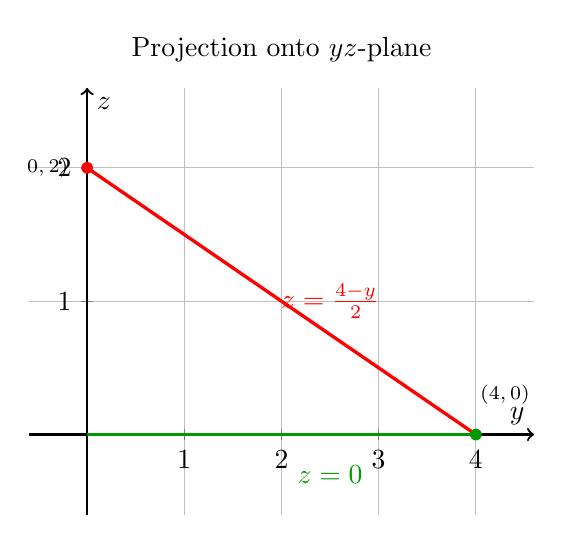
\begin{tikzpicture}
\begin{axis}[
    title={Projection onto $yz$-plane},
    xlabel={$y$}, ylabel={$z$},
    xmin=-0.6, xmax=4.6, ymin=-0.6, ymax=2.6,
    axis lines=middle, axis line style={->, thick},
    width=8cm, height=7cm,
    grid=both,
]
\addplot[red, very thick, domain=0:4, samples=100] {(4-x)/2};
\addplot[green!60!black, very thick, domain=0:4, samples=50] {0};
\node[red] at (axis cs:2.5,1.0) {$z=\frac{4-y}{2}$};
\node[green!60!black] at (axis cs:2.5,-0.3) {$z=0$};
\node[circle,fill=red,inner sep=1.5pt] at (axis cs:0,2) {};
\node[circle,fill=green!60!black,inner sep=1.5pt] at (axis cs:4,0) {};
\node at (axis cs:-0.45,2) {\scriptsize$(0,2)$};
\node at (axis cs:4.3,0.3) {\scriptsize$(4,0)$};
\end{axis}
\end{tikzpicture}
\end{document}